	\subsection{Axe fonctionnel}



\subsubsection{Diagramme de cas d'usage SI Serveur}
\begin{figure}[H]
	\centering
	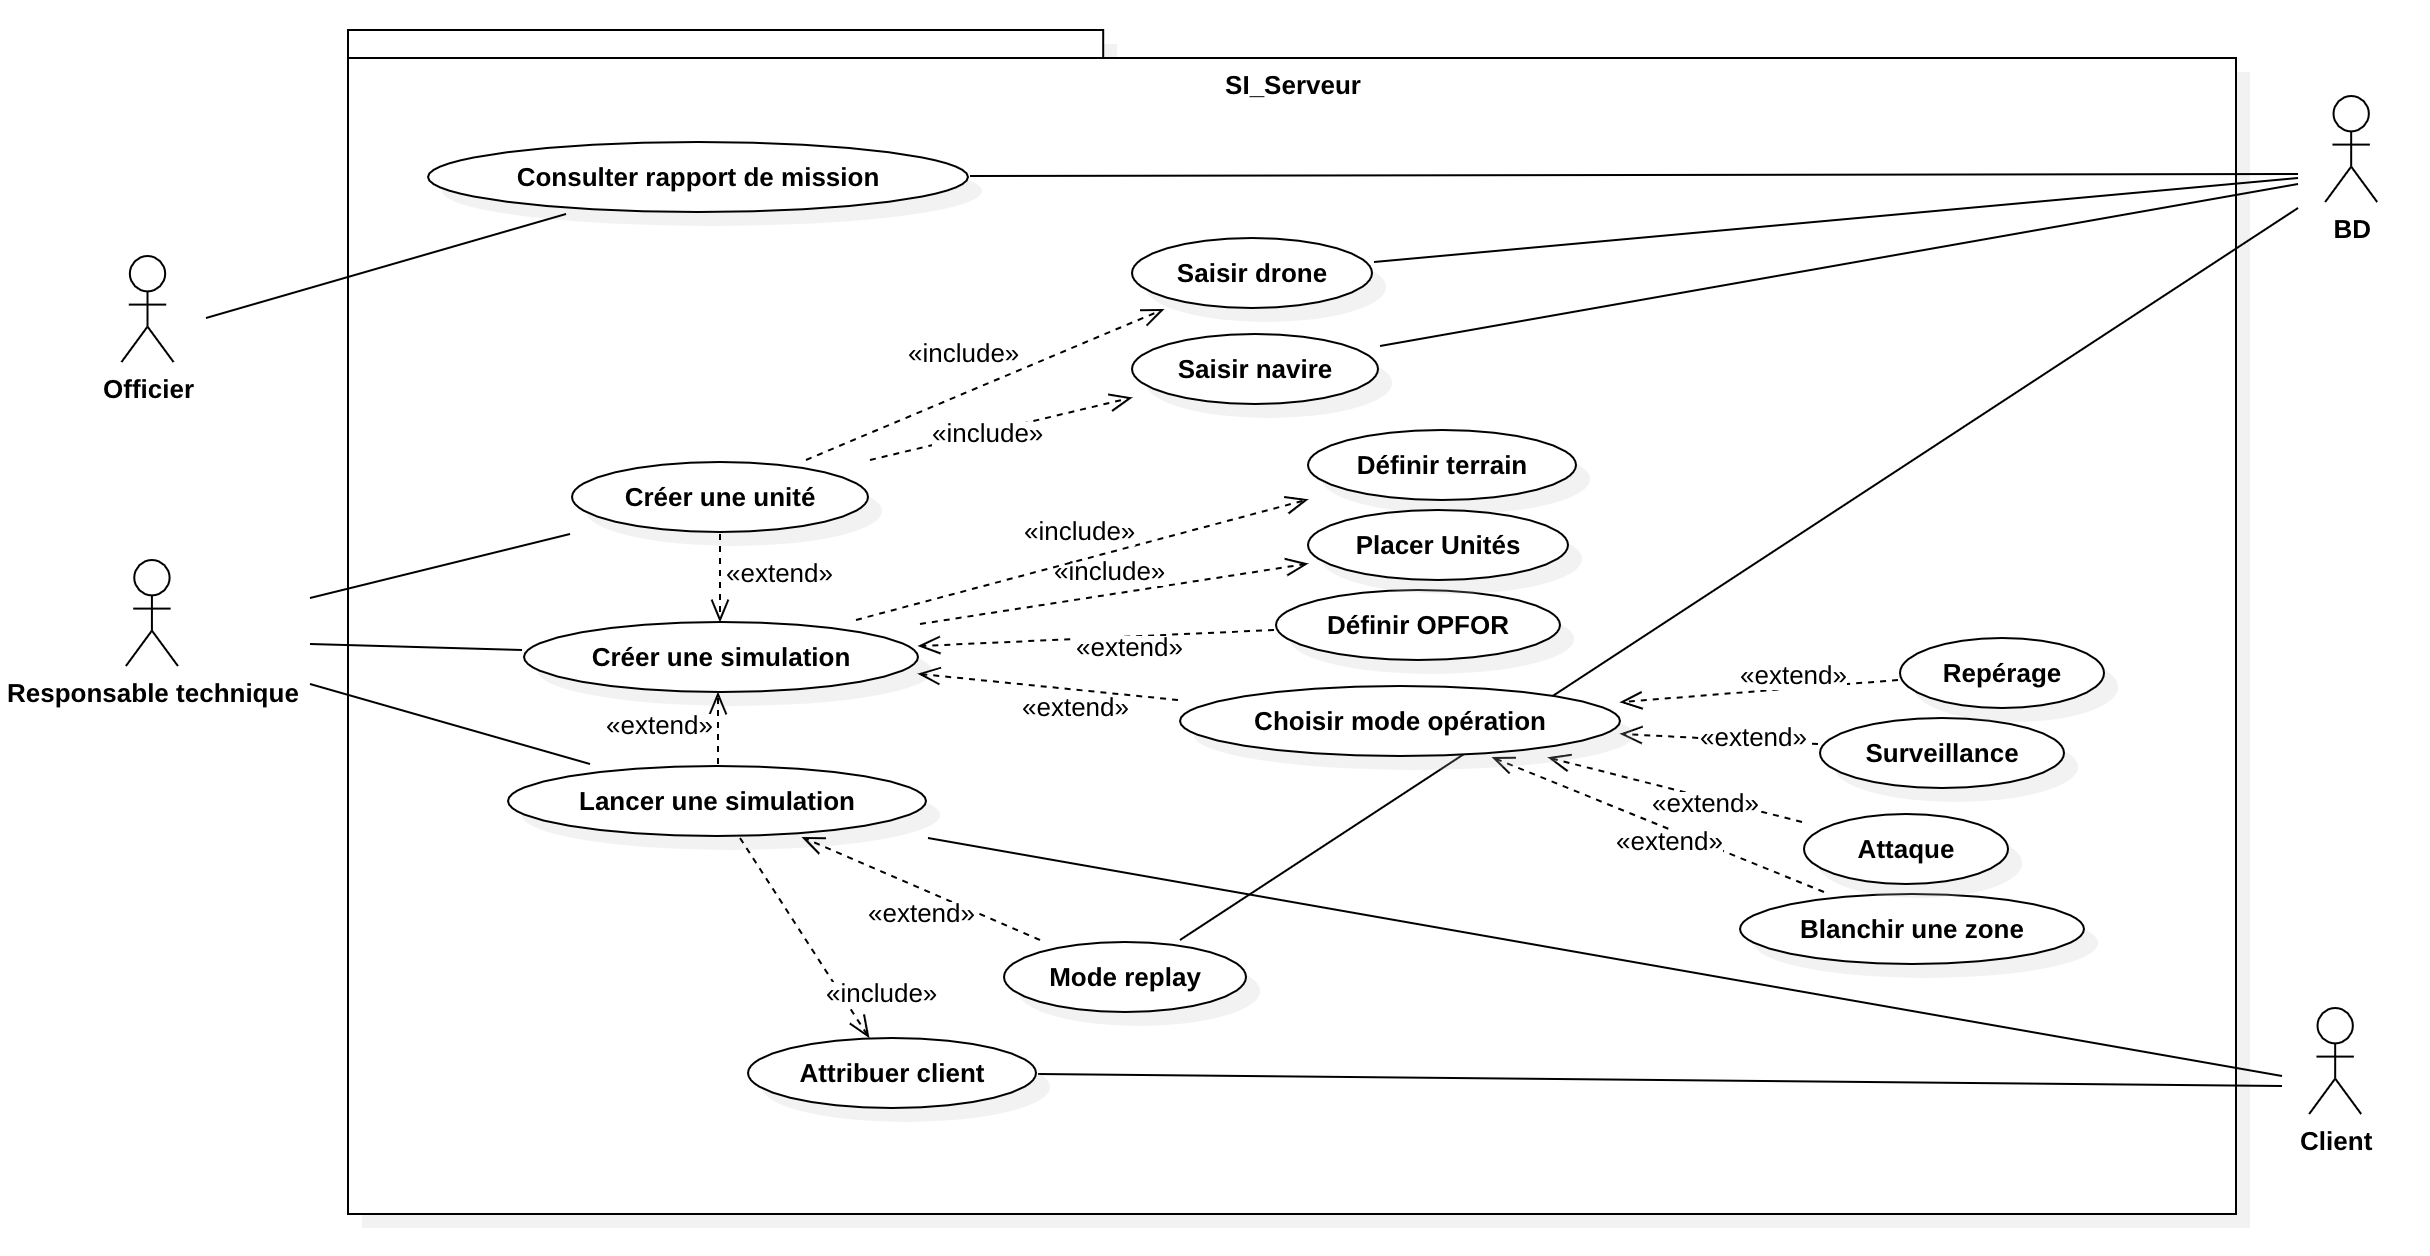
\includegraphics[height=8cm]{img/CUSI_Serveur.png} 
	\caption{CU SI Serveur.}
\end{figure}
\subsubsection{Diagramme de cas d'usage SI Client}
\begin{figure}[H]
	\centering
	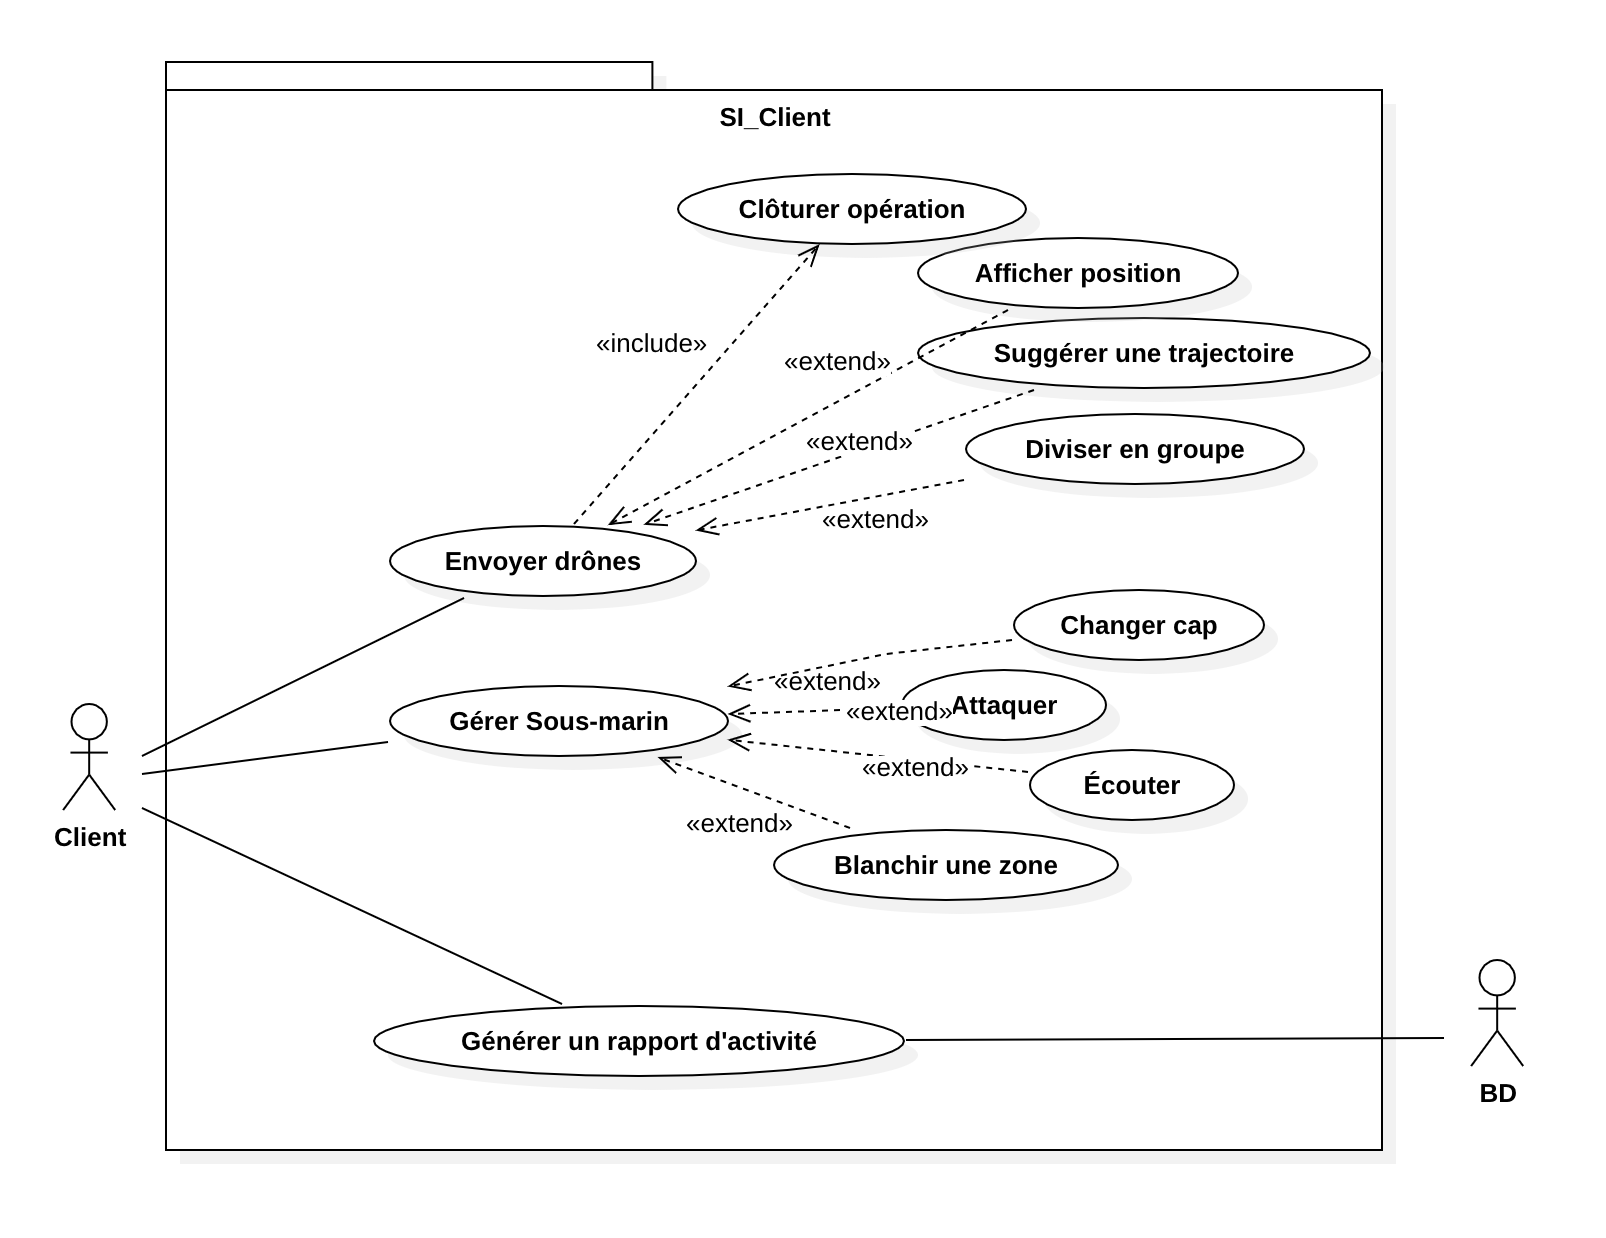
\includegraphics[height=13cm]{img/CUSI_Client.png} 
	\caption{CU SI Client.}
\end{figure}


\subsubsection{Structure du système niveau 1}
\begin{figure}[H]
	\centering
	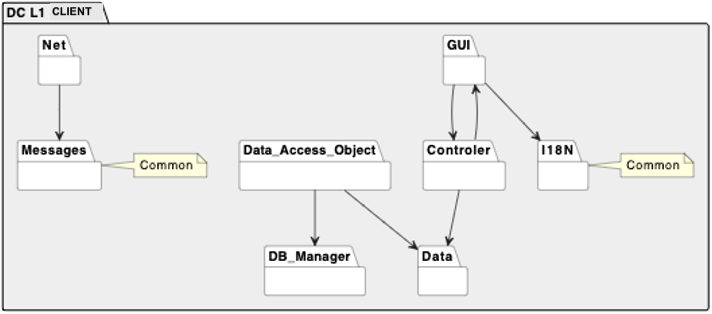
\includegraphics[height=5cm]{img/DC_L1Client.png} 
	\caption{Structure pour le logiciel Client}
\end{figure}

\begin{figure}[H]
	\centering
	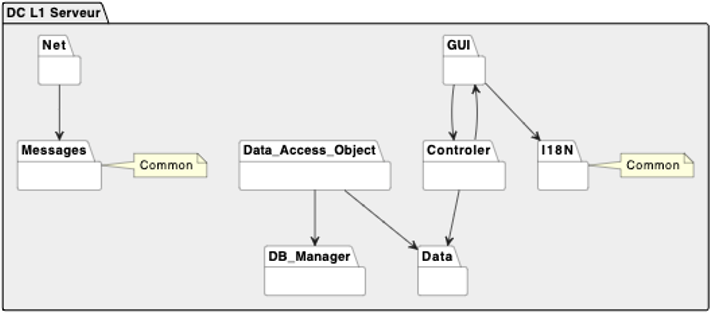
\includegraphics[height=5cm]{img/DC_L1Serveur.png} 
	\caption{Structure pour le logiciel Serveur.}
\end{figure}


\subsubsection{Structure du système niveau 2}
\begin{figure}[H]
	\centering
	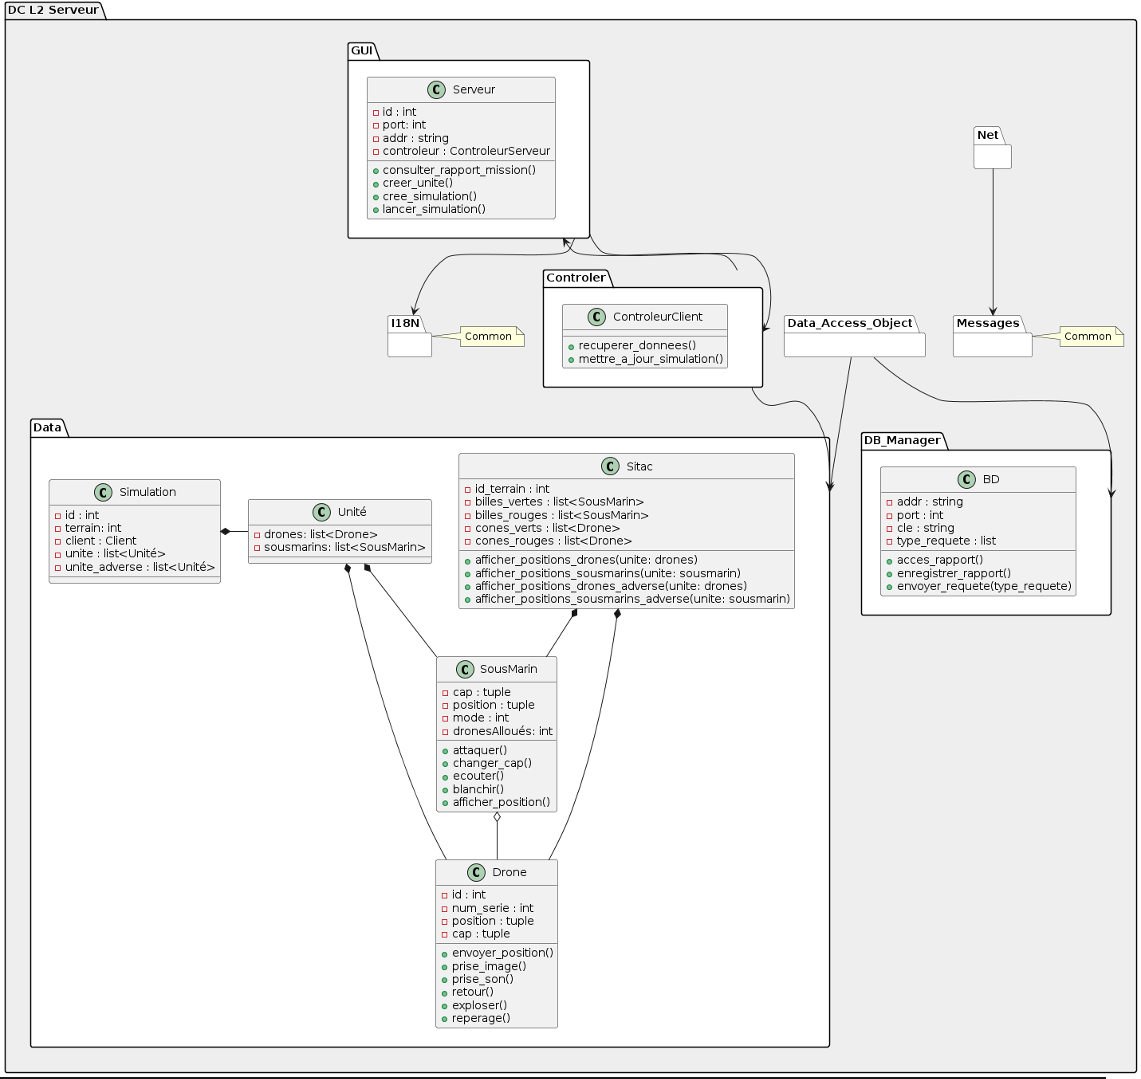
\includegraphics[height=15cm]{img/DC_L2_Serveur.png} 
	\caption{Partie serveur}
\end{figure}

\begin{figure}[H]
	\centering
	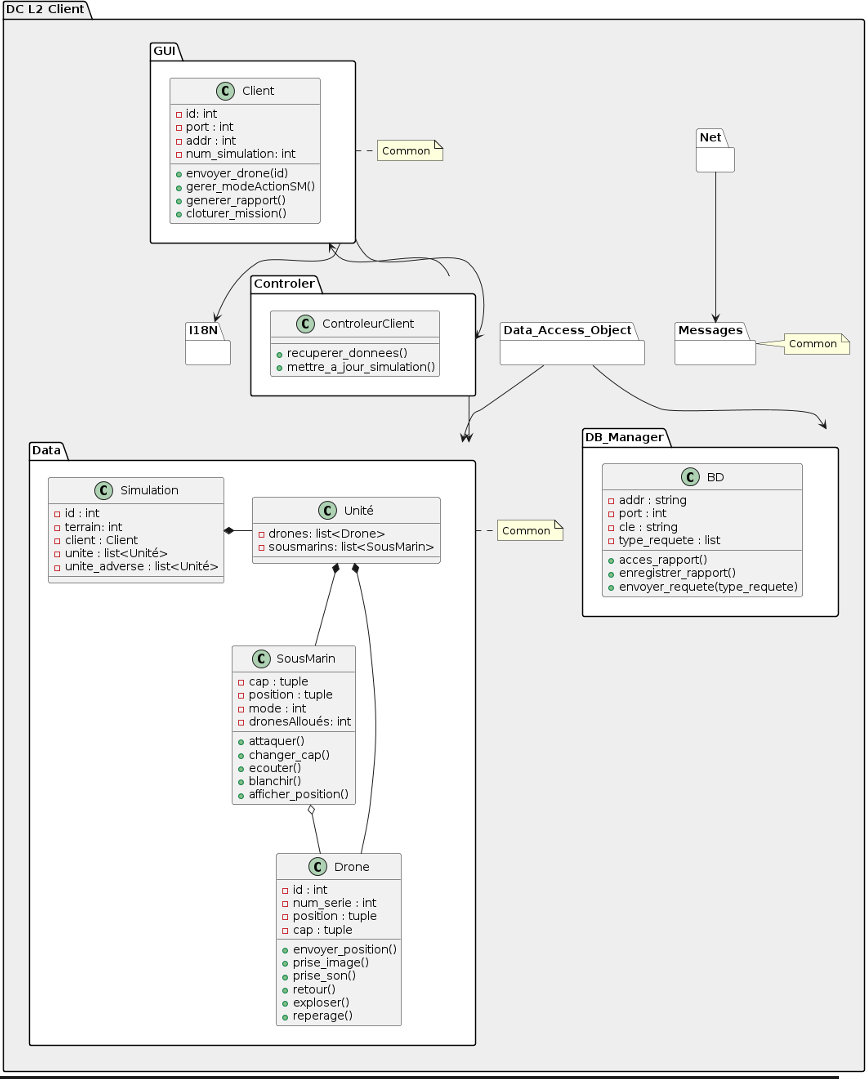
\includegraphics[height=15cm]{img/DC_L2_Client.png} 
	\caption{Partie Client}
\end{figure}



\subsection{Axe statique}
\subsubsection{Diagramme des classes partie Serveur}
\begin{figure}[H]
	\centering
	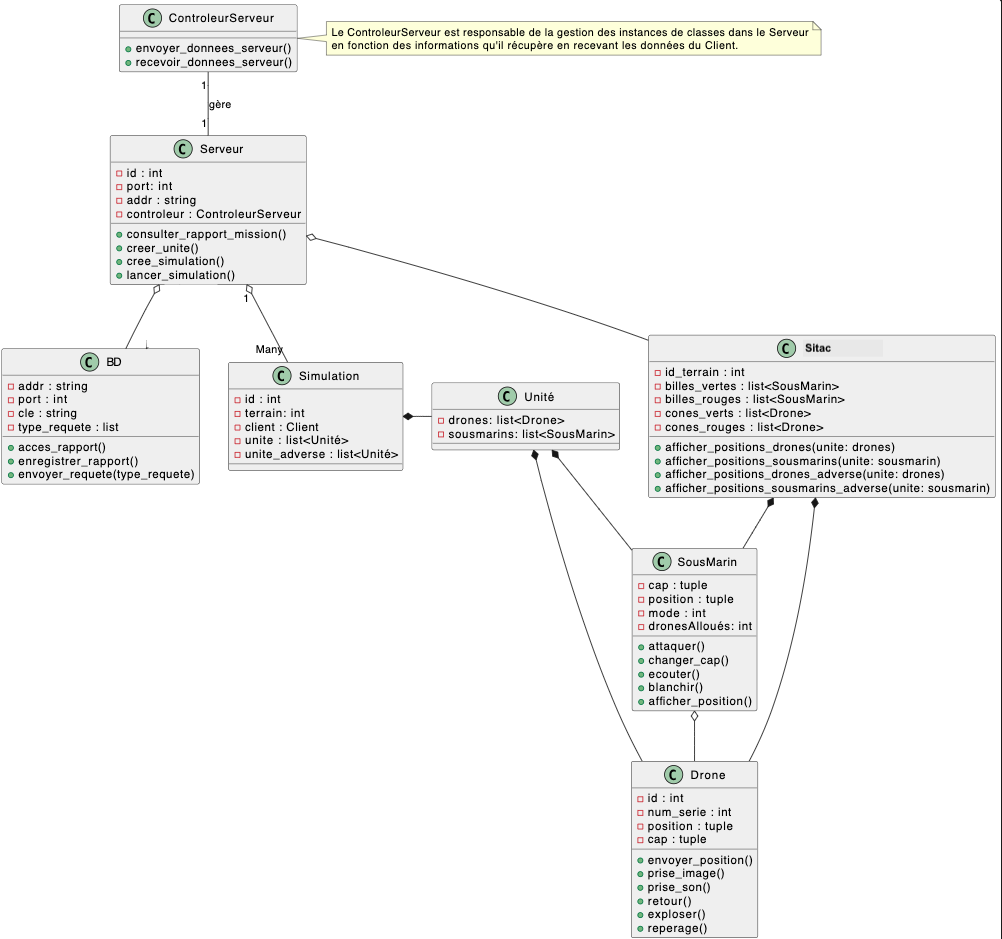
\includegraphics[height=15cm]{img/serveur.png} 
	\caption{Diagramme des classes pour le simulateur partie Serveur}
\end{figure}

\subsubsection{Diagramme des classes partie Client}
\begin{figure}[H]
	\centering
	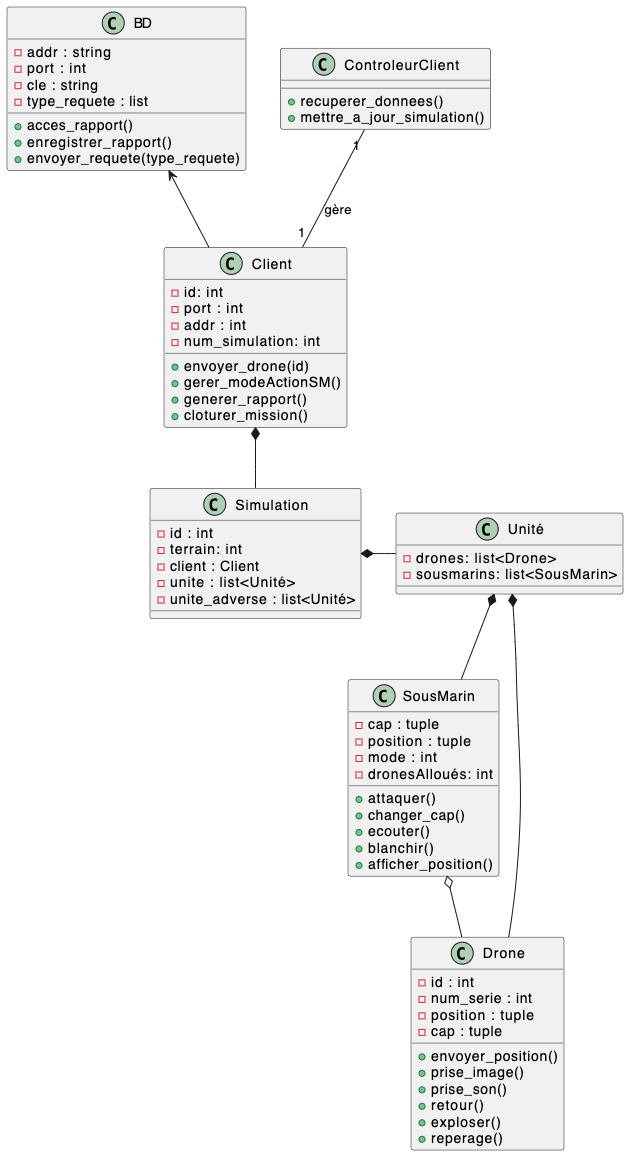
\includegraphics[height=15cm]{img/client.png} 
	\caption{Diagramme des classes pour le simulateur partie Client.}
\end{figure}


\subsection{Axe dynamique}
\subsubsection{Diagramme de séquence Serveur}

\begin{figure}[H]
	\centering
	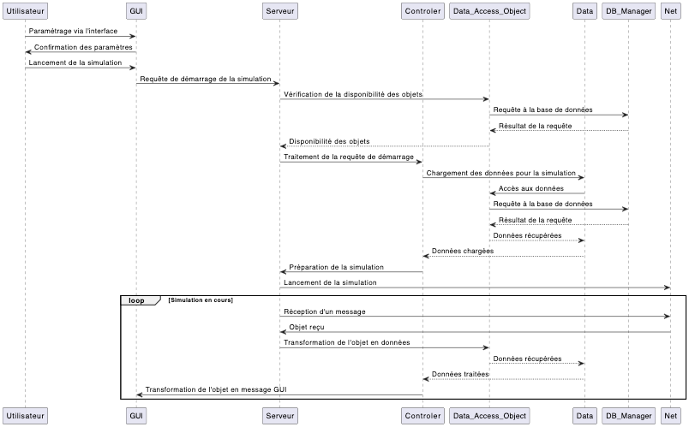
\includegraphics[height=8cm]{img/SeqServeur.png} 
	\caption{Diag. de séq. sur l'intéraction entre le serveur et ses différents composants lors de la configuration d'une simulation.}
\end{figure}

\begin{figure}[H]
	\centering
	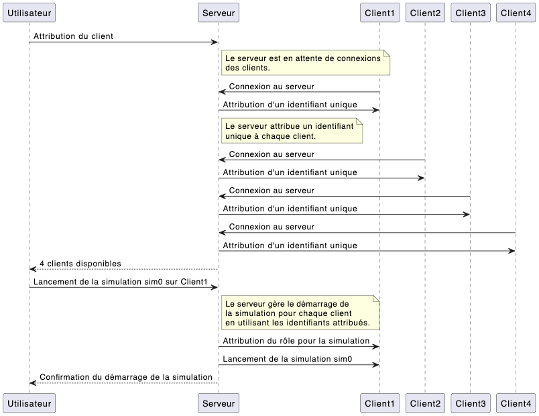
\includegraphics[height=8cm]{img/ServeurRole.png} 
	\caption{Diag. de séq. sur l'attribution des rôles aux clients par le serveur.}
\end{figure}

\subsubsection{Diagramme de séquence Client}
\begin{figure}[H]
	\centering
	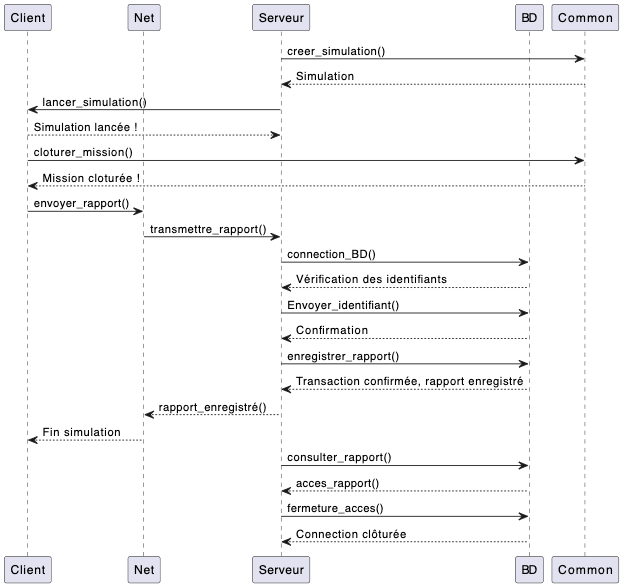
\includegraphics[height=8cm]{img/DiagSeq_IntenvoiRapport.png} 
	\caption{Diag. de séq. pour l'envoi de rapport par le Client}
\end{figure}

\begin{figure}[H]
	\centering
	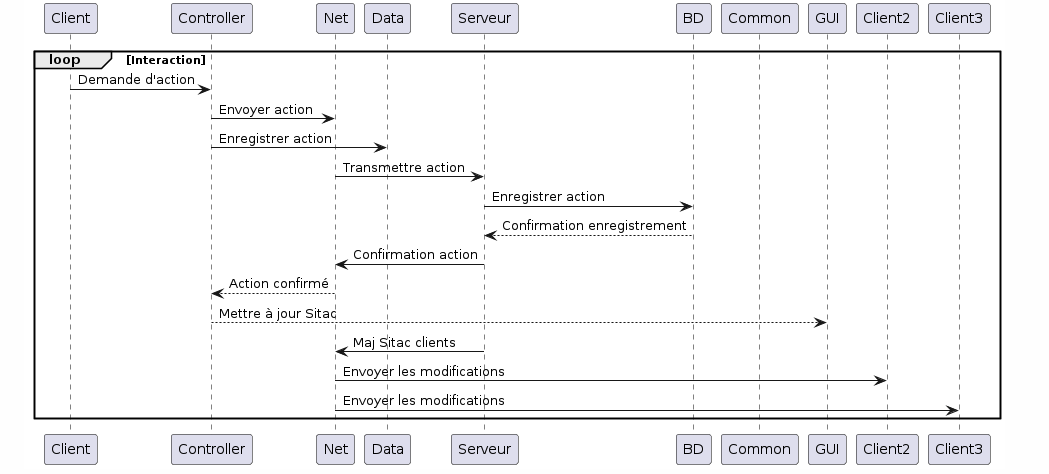
\includegraphics[height=8cm]{img/diagSeqModif.png} 
	\caption{Diag. de séq. pour l'envoi des modifications }
\end{figure}


\subsubsection{Base de donnée: Modèle Entité-Association}
\begin{figure}[H]
	\centering
	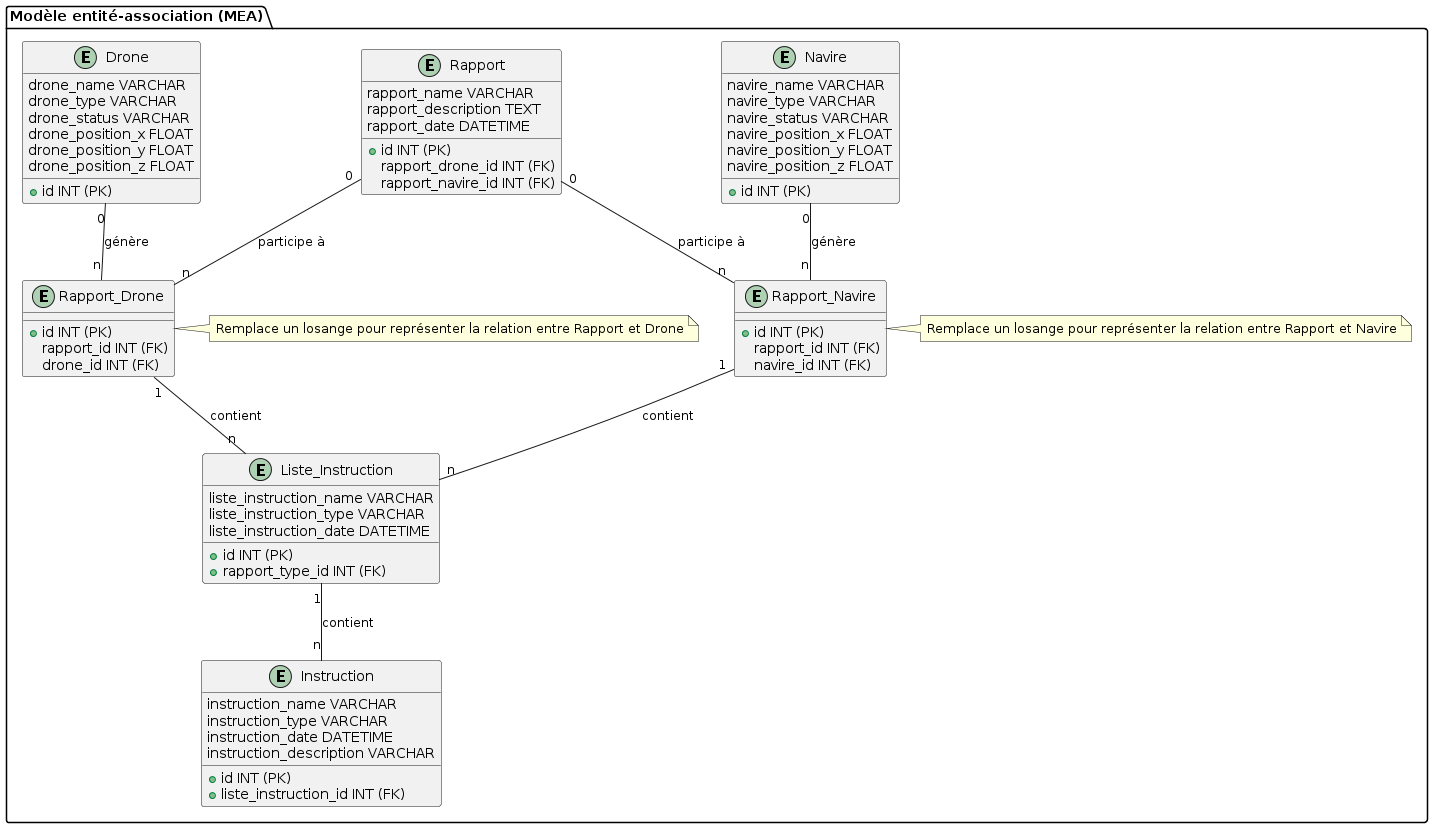
\includegraphics[height=8cm]{img/MEA.png} 
	\caption{MEA pour la BD de Serveur}
\end{figure}

